
% ------------------------------------------------------------
% ------------------------------------------------------------

\section[Summary Plots]{Summary Plots}

\subsection{Scatterplot}
%%%%% New frame
\begin{frame}[allowframebreaks, fragile]
\frametitle{Scatterplots}

To get a quick peak into the numerical variables in the data \ttfamily scatterplot.matrix(): \normalfont
  		\begin{lstlisting}
library(car)		
data(quakes)
scatterplot.matrix(quakes[, 1:4])
		\end{lstlisting}

        \begin{center}
         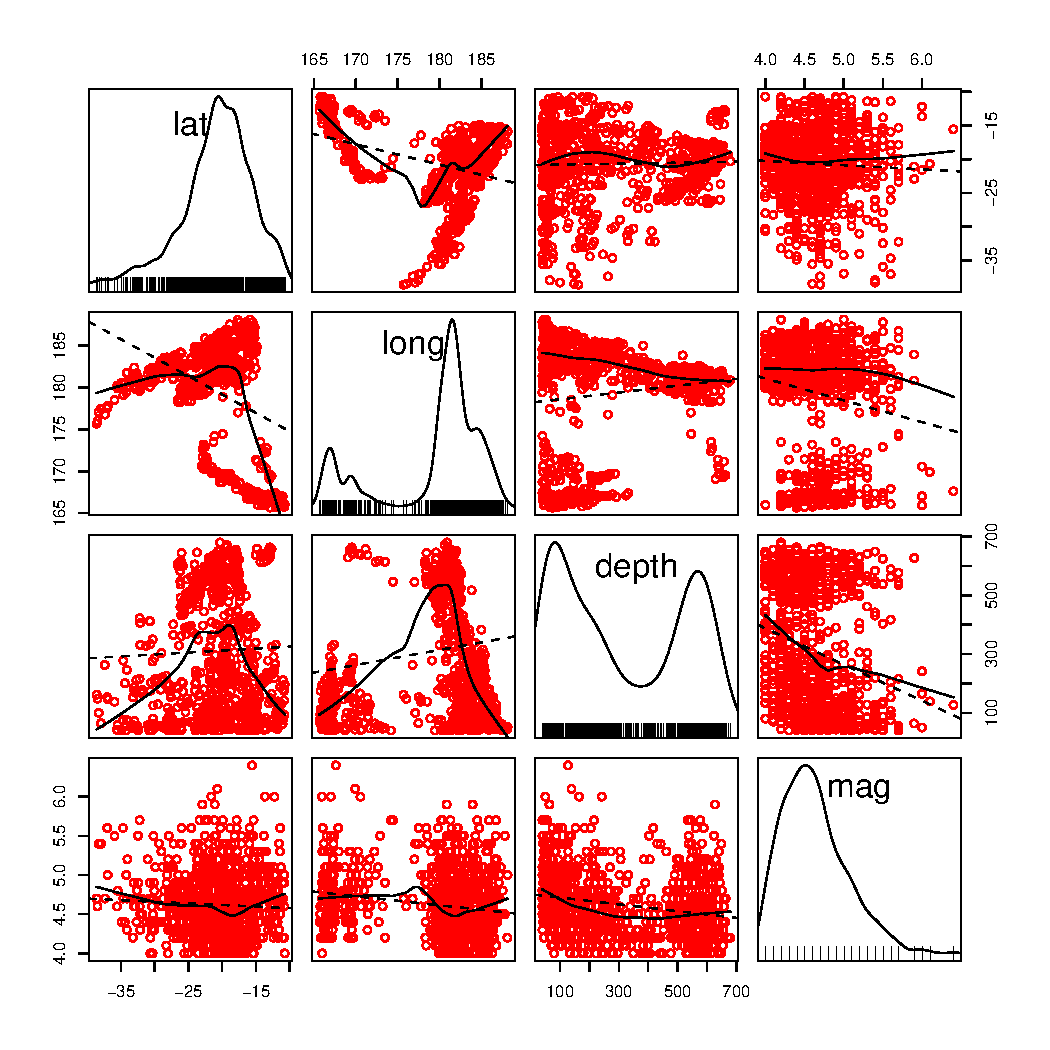
\includegraphics[width=0.63\textwidth]{images/scatterPlot.pdf}
        \end{center}
\end{frame}


%%%%% New frame
\subsection{Histogram}
\begin{frame}[allowframebreaks, fragile]
\frametitle{'Nicer' Histogram}

To compare the frequencies of two variables side-by-side, use \ttfamily beanplot(): \normalfont

	\begin{lstlisting}
library(datasets)
library(beanplot)
data(ToothGrowth)
beanplot(len ~ supp, data=ToothGrowth, col=list(grey(0.5),c(grey(0.8),"white")), border = NA, overallline = "median", ll=0.01, side="both")
legend("bottomleft",fill=c(grey(0.5),grey(0.8)), legend=c("Orange Juice","Ascorbic Acid"))
	\end{lstlisting}
	
        \begin{center}
	         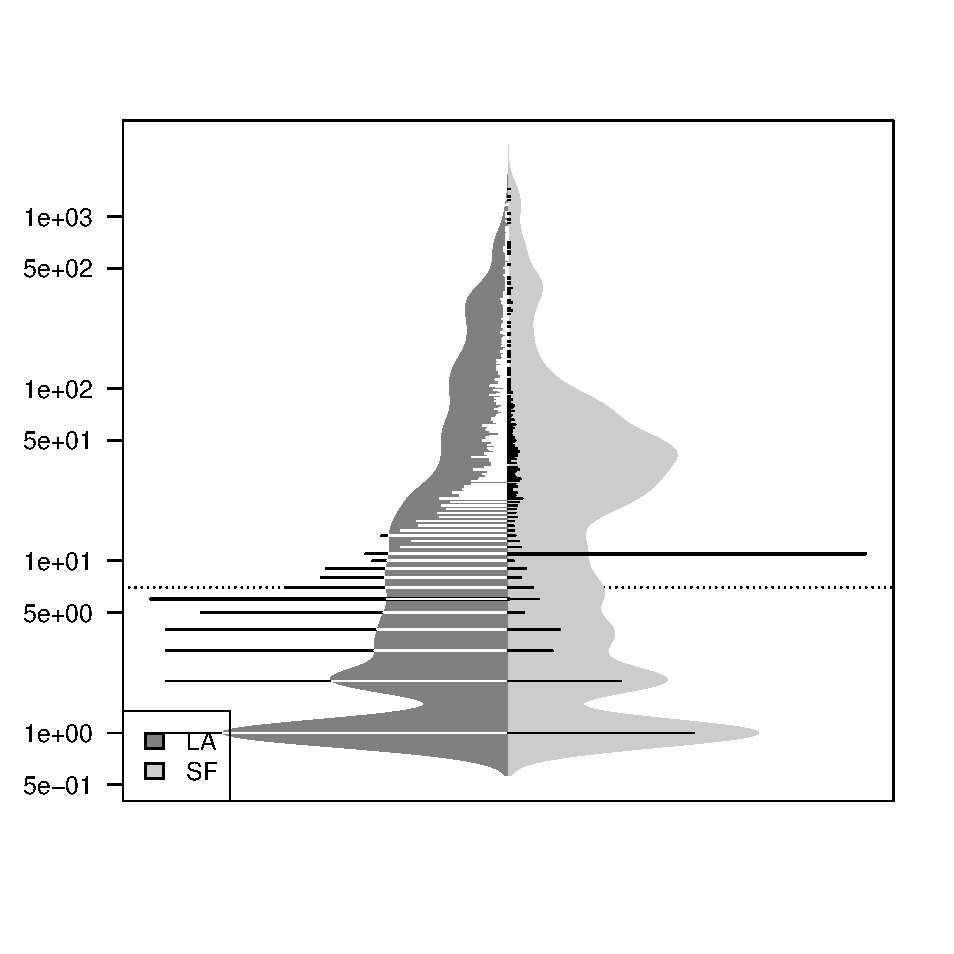
\includegraphics[width=0.65\textwidth]{images/beanplot.pdf}
        \end{center}
\end{frame}

%%% NOT WORK...
%
%library(lattice)
%split.screen(c(1,2))        # split display into two screens
%split.screen(c(2,1),2)      # split bottom half in two
%screen(1)                   # prepare screen 1 for output
%qqplot(ToothGrowth$len~ToothGrowth$supp)
%screen(4)                   # prepare screen 4 for output
% # boxplot(ToothGrowth$len~ToothGrowth$supp)
% beanplot(ToothGrowth$len~ToothGrowth$supp, col=list(grey(0.5),c(grey(0.8),"white")), border = NA, overallline = "median", ll=0.01, side="both")
%screen(1, FALSE)            # return to screen 1, but do not clear
%close.screen(all = TRUE)    # exit split-screen mode


%%%%%%%%%%%%%%%%%%%%%%%%%%%%%%%%%%%%%

% ------------------------------------------------------------
% ------------------------------------------------------------

% Exercise: compare distributions of Iris data
% ID outlier in dataset

\subsection{Exercise I}
\begin{frame}
	\frametitle{Exercise I}
	Compare the distributions of the sepal widths for the three species of irises (using the \ttfamily iris \normalfont data set).
\end{frame}